% !TEX root = ../../Diploma.tex
\section{Parameter Study}
\begin{figure}[ht]
	\centering
	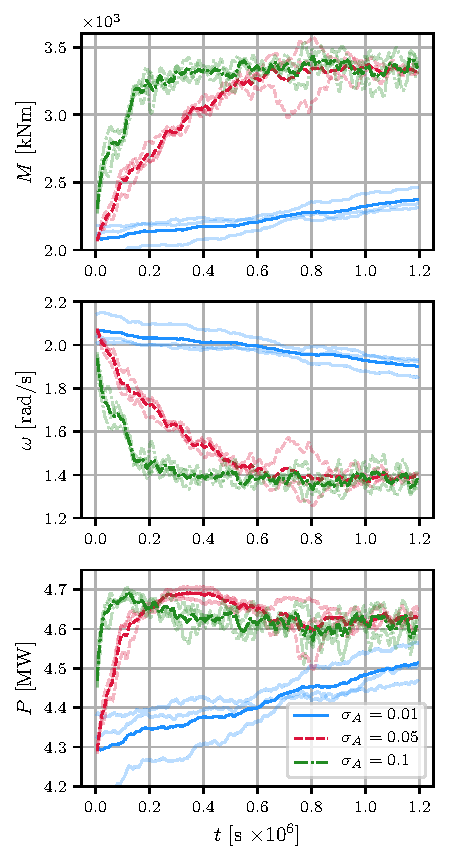
\includegraphics{parameter_study/variance.pdf}
	\caption{$\sigma_A=$ \legendThree{$0.01$}{$0.05$}{$0.1$.}Sensitivity of training to $\sigma_A$. Thin lines are individual trainings, thick lines are the average of all trainings.}
	\label{fig:var}
\end{figure}
To gain insight into the behaviour of the RL-agent and the influence of some of the parameters, a parameter study is conducted. To reduce the effect of the random initialization of the networks, for each tested value of a parameter, three independent agents are trained. The evolution of generator torque, angular velocity and power throughout training for a fixed number of timesteps is compared, since these values are used as action, state and reward, respectively. \\
First the influence of the variance of the action, $\sigma_A$ is studied. The results of the training for agents with variance of $0.01$, $0.05$ and $0.1$ are shown in \autoref{fig:var}. The comparison of the three values shows a clear trend. A higher variance leads to a faster increase in power. 
This can be expected, since a larger variance in the action leads to trying a wider range of actions. Therefore finding a coarse estimate of a beneficial behaviour, that is behaviour that increases the advantage, is more likely. Furthermore it is visible, that the two agents with a higher variance reach similar behaviour. This increases the confidence, that this behaviour represents a local optimum. However, they both reach a maximum of generated power in the first half of training, but are not able to sustain that value throughout the rest of the training. Comparing the different agents with the same set of parameters show that stochastic variation is present in training of the agents.  After around two thirds of training time, one of agents with medium variance shows a significant drop in power, while another performs significantly better than average. However, towards the end of the training, the agents with medium variance perform more similar, more stable and slightly better than the agent with a higher variance. It can therefore be assumed that the choice of variance has to be a balance between a fast increase in the beginning and unstable behaviour in the end. It can be expected that the training of the agent controlling three turbines in the LBM-ALM environment will take significantly more timesteps and the computational cost of a single timestep is also much higher. Therefore, a faster increase is favoured and the variance is chosen to be $\sigma_A = 0.1$. \\
\begin{figure}[ht]
	\centering
	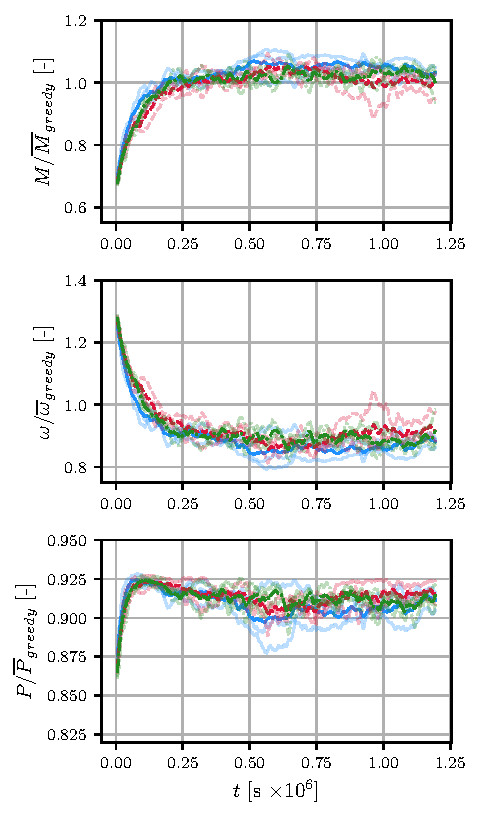
\includegraphics{parameter_study/policy_l2_reg.pdf}
	\caption{$\varepsilon_{p,l_2}=$ \legendThree{$0.0$}{$0.1$}{$0.2$.}Sensitivity of training to $\varepsilon_{p,l_2}$. Thin lines are individual trainings, thick lines are the average of all trainings.}
	\label{fig:p_l2}
\end{figure}
Next, the influence of an $l_2$ regularization of the policy network is examined. The results of the trainings without regularization and with regularization coefficients of $0.1$ and $0.2$ are shown in \autoref{fig:p_l2}. The sensitivity is significantly smaller to this parameter than to an increase in $\sigma_A$. While almost no difference is visible in the beginning for trainings with regularization, no regularization allows for a faster increase in power. However, on average, these agents drop the most afterwards. The agents also differ the most in power towards the end of the training. Remarkably, this is not the case for the generator torque, which differs most for $\varepsilon = 0.1$. To explain this discrepancy in action and reward, looking back at \autoref{fig:cp_+_ct} shows, that $C_P$ is not very sensitive to changes in tip-speed ratio near the optimum. The optimum tip-speed ratio corresponds to an angular velocity of $\omega=\SI{1.58}{m/s}$. \autoref{fig:p_l2} shows that most of the agents operate at angular velocities below the optimum. The aforementioned agent sets a lower generator torque, therefore the angular velocity increases and is actually closer to the optimum. The difference in the case without regularization is caused by an increased torque, which has a bigger effect on $C_P$. In the last third of training, the agents with $\varepsilon_{p,l_2}=0.1$ consistently perform best. Therefore this value is chosen. \\
\begin{figure}[h]%
	\centering
	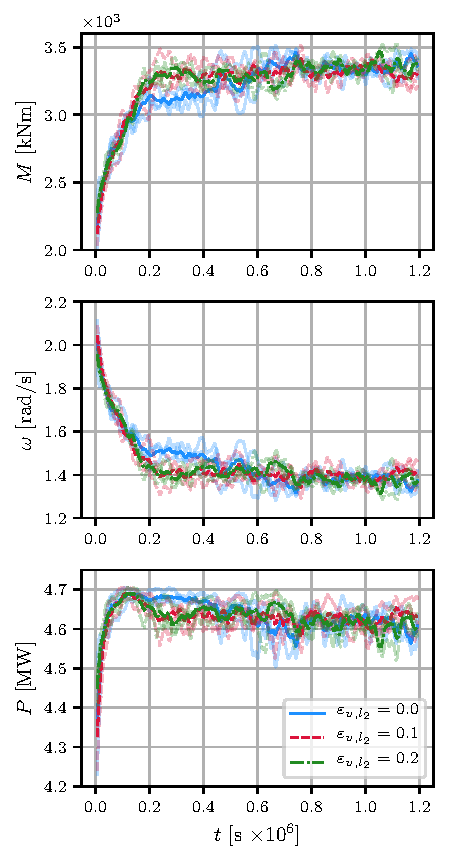
\includegraphics{parameter_study/value_function_l2_reg.pdf}
	\caption{$\varepsilon_{v,l_2}=$ \legendThree{$0.0$}{$0.1$}{$0.2$.}Sensitivity of training to $\varepsilon_{v,l_2}$. Thin lines are individual trainings, thick lines are the average of all trainings.}
	\label{fig:v_l2}
\end{figure}
Finally, the regularization of the value network is tested as well. The same coefficients as for the regularization of the policy network are tested. The sensitivity to a change in this parameter is similar to that of the policy regularization. A noticeable difference between the trainings is a delayed drop for trainings without regularization. However, this is only a delay and later on the reductions in power are of similar magnitude as for the other cases, while the differences in generator torque are even larger than for the other agents. The second half of the training shows no clear trend for the best performance. The differences are small and the none of the averaged values is consistently better than the other. Since none of the tested values offers a clear advantage, the same value as for the regularization of the policy network is chosen.\\
The parameter study revealed a high sensitivity to a change in variance of the action and showed that an $l_2$ regularization benefits stability of the trained network while too much influence of the regularization might inhibit optimization. In general, all of the studied trainings showed that the initial value of the generator torque is significantly lower than the optimal value. This is done by design, since a initial value that is too high leads to slowing down the turbine and a breakdown of $M_{aero}$, which ultimately makes a restart of the turbine necessary. Furthermore, almost all cases showed that $P$ reached a maximum value and then decreased. This was caused by a generator torque that is consistently set higher than what would be expected from a comparison with the controller curve of the greedy controller in \autoref{fig:controller_curve}. It can also already noted that a lot of simulated time is necessary for the training of the agent. It can be expected that the necessary time will be at least similar, probably more for the training of an agent controlling three turbines.
